\documentclass[a4paper]{report}
\usepackage[brazil]{babel}
\usepackage{graphicx}
\usepackage{imakeidx}
\usepackage{lettrine}
\usepackage[notlof]{tocbibind}

\makeindex[columns=3, title=keywords, intoc]

\title{Verde e Brutall}
\author{el comodin - smvb}
\date{agosto 2017}

\renewcommand*\contentsname{idx} 

\begin{document}
 
\maketitle
 
\tableofcontents

\clearpage

\addcontentsline{toc}{section}{o verso}
\section*{janela aberta}

\lettrine[findent=2pt]{\fbox{\textbf{E}}}{ }ssa \'e a saga\index{saga} de um encontro com a maquina, escrita por um motorista, e narrada por um autom\'ovel 
fabricado no brasil, desenhado por uma garota, filha de um empresario carioca, que administrou a f\'abrica de
 implementos agricolas e ferroviarios em Entre Rios.

A saga brasilis da injambra e do espirito criativo\index{criativo} aliada a emo\c{c}\~ao

Diversas aventuras, que ao longo do tempo vivenciei, me deram a ideia de 
registrar as coisas mais interessantes, pois sei que daqui pra frente vai ser cada vez mais dif\'icil algu\'em vicenciar, por diversos motivos, a modernidade e complexidade gradual dos meios de transporte dispon\'iveis, a propria
natureza humana de querer sempre facilitar, abstrair e afastar-se ao m\'aximo possivel de saber como as coisas funcionam, da aventura do risco e do instinto\index{instinto}.

Pra mim, \'e isso que significa um autom\'ovel antigo, afastar um passo do materialismo, de querer sempre o carro do ano, da moda, da preocupa\c{c}\~ao natural de nossos dias
e aproximar do natural, do divertido, do instinto e de tudo que da gra\c{c}a a vida, a aventura, a emo\c{c}\~ao.

E n\~ao sou o \'unico que pensa assim, vide mujica, grande mestre do nosso tempo que nao me deixa mentir \dots

\'E disso que se trata esse livro, o prazer da vida contado por uma maquina de 6 cilindros\index{6 cilindros}, 4 rodas e um cora\c{c}\~ao.

Agrade\c{c}o a todos os amigos(as) que fizeram parte desta aventura, e desde j\'a dedico esta obra a todos voc\^es.

\clearpage

\addcontentsline{toc}{section}{descoberta}
\section*{A descoberta}
Nos anos 80, quando eu tinha meus 11 anos, havia uma santa matilde\index{santa matilde} branco perolada na minha cidade,
eu passava por ela algumas vezes, indo ou voltando da escola, sempre achei o carro mais bacana de todos\dots

\addcontentsline{toc}{figure}{o sm branco}
\begin{figure}[!htb]
\centering
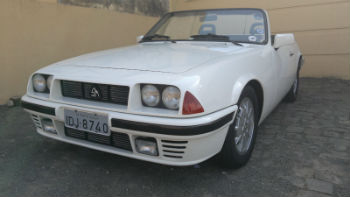
\includegraphics{sm_bco_per}
\caption{SM branco Perolado}
\label{sm_bco}
\end{figure}

Esta id\'eia fortaleceu na minha mente, quando em meados dos 80 o filme "devolta para o futuro" chegou aos cinemas, naturamente como todos nessa \'epoca
fui assistir e como amante de tecnologia e fic\c{c}\~ao fiquei encantado pra n\~ao dizer, abestado por aquele delorean, naturalmente a imagem da SM perolada
voltou para minha cabe\c{c}a como sendo o mais proximo que eu podia achar no brasil de uma. Salvo \'e claro os detalhes t\'ecnicos da viagem no tempo q requer
a lataria exposta para conduzir os 1.21 GigaWats pela superficie permitindo o deslocamento temporal \dots

Certo dia, pela manh\~a, seu Louren\c{c}o, meu falecido pai, me pediu para ligar o carro, um ford scord ghia, para aquecer o motor.

Mesmo n\~ao sendo necess\'ario para um carro relativamente moderno para \'epoca, para mim foi uma experi\^encia \'unica,
at\'e aquele momento, eu nunca havia ligado um carro, pra mim foi um divisor de \'aguas para a vida adulta.

Obviamente eu n\~ao fazia ideia do funcionamento da embreagem e da marcha, liguei o carro com a marcha engatada e por sorte
nao demoli a frente do carro, foi a unica e ultima vez que tive a chance de fazer aquilo, mas a emo\c{c}\~ao do motor ligando ficou
na minha mem\'oria. 

Naquele mesmo ano vi mais algumas vezes a SM branco perolado e pensei que se algum dia eu pudesse ter um
autom\'ovel, seria uma SM, esse dia chegou em 2011.
\clearpage
Eu estava visitando uns amigos em rio grande e fui convidado para almo\c{c}ar \`a bordo com a tripula\c{c}\~ao do Atl\~antico Sul.

\addcontentsline{toc}{figure}{atl\^antico Sul}
\begin{figure}[!htb]
\centering
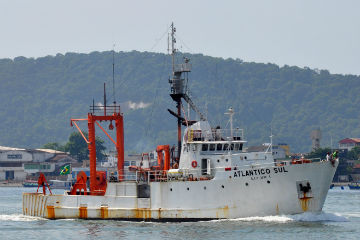
\includegraphics{atsul}
\caption{Navio oceanogr\'afico da FURG}
\label{at_sul}
\end{figure}

Durante o almo\c{c}o o assunto se dirigiu para autom\'oveis, lembrei do meu antigo sonho e compartilhei com o pessoal, nesta ocasi\~ao um dos marinheiros
me falou que havia uma santa matilde a venda em tapes, um conhecido.


Durante o almo\c{c}o o assunto se dirigiu para autom\'oveis, lembrei do meu antigo sonho e compartilhei com o pessoal, nesta ocasi\~ao um dos marinheiros
me falou que havia uma santa matilde a venda em tapes, um conhecido.

Durante o almo\c{c}o o assunto se dirigiu para autom\'oveis, lembrei do meu antigo sonho e compartilhei com o pessoal, nesta ocasi\~ao um dos marinheiros
me falou que havia uma santa matilde a venda em tapes, um conhecido.

Meu amigo Stefan, que havia convidado para o almo\c{c}o com sua equipe de trabalho, entusiamou-se com a informa\c{c}\~ao, e eu tambem, obviamente, e na semana 
seguinte fomos com mais um amigo de rio grande, Daniel Torres, vulgo "bala", outro entusiasta dos 6cilindros, ver a preciosidade.

Durante o trajeto, rio grande - tapes, conversamos muito, sobre os motores, a divers\~ao, pescarias, mas o que nao saia da cabe\c{c}a, a SM.   
\clearpage

\addcontentsline{toc}{section}{primeira vinda}

\section*{primeira vinda}

Era verde, assim como seu interior, perfeita, parecia tudo ok quando vimos, exceto os pneus, esses estavam na capa da gaita

\addcontentsline{toc}{figure}{273a sm}
\begin{figure}[!htb]
\centering
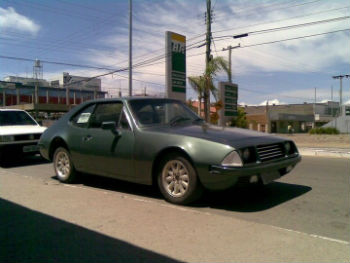
\includegraphics{sm273}
\caption{273$^{a}$SM fonte: Cadastro Nacional da Santa Matilde}
\label{a 273a SM}
\end{figure}
\clearpage


\addcontentsline{toc}{section}{4marchas (v)arretado}
\section*{4marchas (v)arretado}

Ela veio com cambio manual 4 marchas, \'e meu primeiro carro, adorei. Havia um click em cada marcha,
mais tarde num posto no cassino meu camarada Daniel torres me mostrou por que, o cambio era exposto!
Uma serie de alavancas mexiam diretamente nas engrenagens, essas dimensionadas pra nao faltar as demais 
marchas, a 3a era extremamente poderosa, e a quarta parecia ser mais leve que uma sexta, andava muito. 
Mas nao consegui aproveitar o suficiente eu acredito, passei uns 2 anos assim e percebi que o fato de 
acavalar as marchas deixava o auto pouco confi\'avel e optei por botar uma caixa de 5 marchas mais 
moderna.
Certamente foi a coisa que eu mais tenho saudade, acredito que todos que tiveram esta oportunidade 
se lembram dessa caixa de 4 marchas varetada.

\addcontentsline{toc}{figure}{4 marchas opala varetada}
\begin{figure}[!htb]
\centering
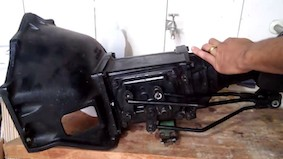
\includegraphics{caixa4}
\caption{caixa 4 marchas com click. fonte: google}
\label{4 marchas opala varetada}
\end{figure}
\clearpage


\addcontentsline{toc}{section}{fan clube}
\section*{fan clube}

Ao longo do tempo em que utilizei a santa matilde surgiram f\~ans um exemplo \'e este pessoal da unissinos, \footnote{http://www.budanga.com.br/2012/06/o-pessoal-hoje-eu-tava-chegando-no.html} 
Nesta mesma \'epoca um acontecimento inusitado colaborou para a iniciativa de escrever as aventuras.

\addcontentsline{toc}{figure}{inicio do fan clube}
\begin{figure}[!htb]
\centering
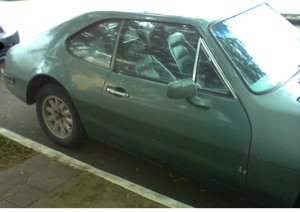
\includegraphics{Foto0296}
\caption{pessoal da unissinos fonte: www.budanga.com.br}
\label{fan clube SL }
\end{figure}


\addcontentsline{toc}{figure}{fan clube tecnosinos}
\begin{figure}[!htb]
\centering
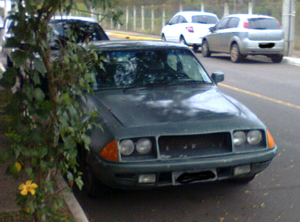
\includegraphics{Foto0295}
\caption{pessoal da unissinos fonte: www.budanga.com.br}
\label{Blog do pessoal da Tecnosinos }
\end{figure}
\clearpage

\addcontentsline{toc}{section}{o destino, eh o caminho, nocoes de proposito}


\section*{festivais}
	muitos planos para os festivais, carros antigos lembram eventos mais tribais, e isso na verdade sao os festivais de hoje em dia, 
        estamos em outubro de 2019 proximo mes havera um festival no qual a verde e brutal conhece bem, ja trabalhou duro, caiu em valetas
        foi rebocada por fitas de e saiu mais feliz 

\section*{acampamentos}
	existe um vies filosofico no quesito acampamentos, este eh o proposito primordial no qual eu investi meu tempo para obter o dinheiro necessario para possuir uma maquina que me facilite esta atividade


 
\addcontentsline{toc}{section}{nova forma de acelerar}

\section*{nova forma de acelerar}

Precisei criar esta alternativa na saida de um aniversario, estava em S\~ao Leopoldo, na casa de uma colega de trabalho, curtindo um bolo e papeando com os colegas
Tava divertido, mas na hora de ir embora percebi q estava sem acelerador, achei estranho e verifiquei no carburador que o cabo estava partido a 5cm dele.
Ai imaginei algo, havia um barbante de nylon no porta malas, se eu pudesse deixar uma fresta no capo eu poderia usar esse cord\~ao para acelerar pela janela, poupando uns 200 reais de guincho.
E foi o que eu fiz, no come\c{c}o foi meio estranho coordenar a embreagem, mas duas lombadas depois eu ja tinha pegado a manha.
Voltei tarde da noite de S\~ao Leopoldo para Porto Alegre acelerando por um barbante preso no carburador direto pela janela.
Ahhh o mais importante, para nao ficar presa a corda deixei um pano preso na fresta do cap\^o deixando espa\c{c}o suficiente para n\~ao trancar acelerado. 
acontecido em 1 de fevereiro de 2011 verificar ano

\addcontentsline{toc}{section}{TODO}

\section*{prot\'otipo e ideias soltas}
Uma coisa que eu notei \'e q me senti livre para criar pois sabendo como funciona eu facilmente posso adaptar algo e nao ficar na m\~ao


\section*{caseiro do sitio shambala}


Janeiro de 2018, meu grande amigo canadense sr. gersteimer ( vulgo dr. gonzo) me chamou pra tomar conta do seu sitio em viamao durante suas ferias de inverno, aproveitei pra levar a SM pra passear e fazer alguns pequenos reparos na porta do motorista enquanto curto um pouco de natureza, fogueiras, uma cachorrada marota e o novo amigo Valentin ( o cavalo da tes, filha deste meu amigo) foi um m\^es divertido com varias idas e vindas com a santinha, ela se comportou divinamente, sou muito feliz por poder rodar com esse carrinho. 


\section*{devotos da santa matilde}

Agosto de 2018, fazem meses que nao rodo com a santa matilde, puro desleixo mesmo, h\'a meses tenho combinado com o amigo Lee Ohn ( se eu for contar as historias com esse camarada da quase outro livro ) de subtrai-lo de um gerador que esta ocupando espa\c{c}o na casa dele, e finalmente chegou o dia, aproveitei uma folga no meio da tarde para evadir o transito que esta cada vez mais ca\'otico nesta porto alegre e fiz a miss\~ao, a matilde estava coberta de p\'o, estava parada desde janeiro, mas incrivelmente um xorinho de supra direto no carburador e ela ronronou sem muito trabalho, fizemos a mao de carregar o gerador, e meu amigo virou mais um devoto da santa, aproveitei e mostrei como fazer uma liga\c{c}\~ao direta, ta na hora de consertar isso, mas nao consigo, funciona t\~ao bem e \'e t\~ao legal que mesmo tendo comprado os componentes para modernizar eu nao me presto a finalizar o trabalho. 

\clearpage

\printindex
 
\end{document}
